\documentclass{../notes}

\title{直播助农场景下消费者的产品质量敏感度与产品信任的建立机制调节}

\begin{document}
    \maketitle

    \section{研究背景}

    随着互联网技术与基础设施的发展,网络视频与视频直播成为一种新的在线内容表现形式。其中视频直播因其实时性及真实性获得了电子商务平台的青睐。自2019年起,京东、淘宝、天猫等电商平台均上线了视频直播的功能。在直播过程中,商家可以介绍、演示产品,与消费者实时互动,同时消费者也可以通过弹幕等多种互动形式与在线购买的其他消费者互动。在消费者作出消费之前,消费者通过主播的实时演示和其他消费者的互动,在作出消费前就已经初步建立对产品的信任,推动了消费者的消费行为,有效提高了电子商务平台上产品的销量。截至2021年,我国已有超过4亿人参与电商直播消费,直播电商交易规模已占网络零售交易总量的17.97\%,直播已经成为电商平台上一种重要而行之有效的营销形式\cite{noauthor_2021}。
    但相关研究表明, % TODO 补充文献说明直播销售的退货率较高
    通过视频直播销售的商品有较高的退货率\cite{gong2021, liu2021}。一方面,在直播带货的场景下,消费者与直播间的其他消费者积极互动,由此作出的消费在一定程度上受到其他消费者的影响,属于“冲动消费”;另一方面,直播带货虽然通过视频直播这一机制初步建立了消费者对产品的信任,但并未消除消费者对产品质量的敏感度,因此当消费者买到了质量不符合预期的商品时,消费者仍然会选择退货。因此,消费者对产品质量的敏感会影响消费者建立产品信任,进而影响产品的营销推广。

    助农直播是以帮助中小型农户销售农牧产品的直播形式。相较于传统的农产品市场,由于助农直播在农户与消费者之间建立了点对点的供求关系,农户拥有自主议价权,不再需要层层的批发商进行转运,降低了供应链造成的溢价。因此借助于助农直播,农户能够达到更多的收入。另一方面,传统的农产品市场由于受到供求关系波动的影响,会存在供大于求的风险。而农产品不同于其他工业化生产的产品,其保质期较短,若超过保质期则会全部损失,受到供求关系失衡的冲击更大。而直播助农扩大了农户潜在的消费者,有助于在农产品丰收时帮助农户消解超额的农产品。

    由于中小型农户的资金水平、技术水平往往不高,对直播技术、相关营销手段了解较少,直播助农通常由公益性企业或地方政府进行背书,对农户进行资金、流量等资源上的补助与技术上的指导。但由于个体农户独立经营,在生产过程中往往难以实现高水平的产品质量控制流程。同时由于新鲜农牧产品的保质期通常较短,产品需要在短时间内运达消费者手中,但农村的运输条件较差,使得直播助农中销售的农牧产品的质量相较于大型企业工业化生产的产品较差,缺乏产品质量的竞争力优势。另外,直播助农还有另一方竞争对手,即传统的线下的农产品市场。在线下的农产品市场中,消费者可以对农产品的质量有直观的体验,并尽量挑选其中质量好的购买。因此即使助农直播能够以更低的价格为消费者提供农产品,对助农直播产品缺乏信任会影响消费者的购买决策。此外,若消费者对某一个直播助农商家产生了不信任,该消费者对其他直播助农商家的信任度也会下降,最终使得该消费者完全拒绝通过直播助农渠道购买农产品。

    综上所述,如何在消费者对产品质量较为敏感的环境下,建立消费者对产品的信任,是当前直播助农较为关键的问题。目前直播助农的商业模式中,直播间的互动内容与消费后的消费者评价相互独立。即,进入直播间的消费者并不了解商家所推介商品的品质。若将其他消费者的消费评价引入直播助农的互动内容中,会使消费者对产品的品质产生直观的感受,从而调整对产品品质的预期,建立对产品的信任。本文希望研究,将直播助农的消费者评价反映到直播画面或直播弹幕中,是否对消费者建立对销售产品的信任有帮助,从而提高直播助农的产品销量。

    \section{相关研究回顾}

    本节从直播电商、直播互动等角度对相关研究进行了回顾。

    \subsection{直播电商}

    目前,由于直播电商这一营销模式逐步走向成熟。在新冠疫情的大背景下,直播电商能够克服传统线下批发商、零售商受到疫情导致的消费者流动限制,最大限度地帮助农户及零售商销售产品。郭红东等人调研了直播助农发展的可持续性,研究结论表明,由于目前农村地区的供应链不完善,使得直播助农主要通过较低的价格等手段换取更高的销售量,而较低的价格最终会影响到直播助农的效果;另外包含直播助农在内的整个直播电商存在管理机制尚不完善的问题,市场上出现的低质量产品会降低消费者对直播助农的信任,从而影响直播助农的效果\cite{guo2020}。刘忠宇等人使用扎根理论,对直播电商中消费者购买意愿的形成机制进行分析,研究表明,网络直播在消费者认知维度(主播层面)、情感维度(群体认同与参与感)与意动维度(购买选择)三个方面推动消费者的购买行为\cite{liu2020}。熊雪等人从中介能力的角度分析了农产品电商直播中消费者信任的形成机制\cite{xiong2020}。

    \subsection{直播互动}

    实时互动是视频直播相较于在线视频的一大优势。在电商直播中,主播与消费者之间合理恰当的互动可以促进消费者的购买意愿,提高直播间的销量。郑兴等人从主播的互动类型出发,使用S-O-R模型分析了互动类型对消费者消费购买意愿的影响,研究表明主播与消费者的积极互动可以通过增强消费者的心流体验提高消费者的购买意愿,同时关系导向型主播对消费者购买意愿的影响效应更强\cite{zheng2019}。除了消费者与主播之间形成互动关系增强消费者购买意愿意外,研究者还对电商直播中消费者之间以实时弹幕为载体的互动形式对消费者消费意愿的影响。蒋芮等人使用柯林斯的互动仪式理论分析了电商直播中的消费者互动对用户消费的影响\cite{jiang2020}。

    \section{研究模型与假设}

    本文的研究模型如图\ref{fig:1}所示

    \begin{figure}
        \centering
        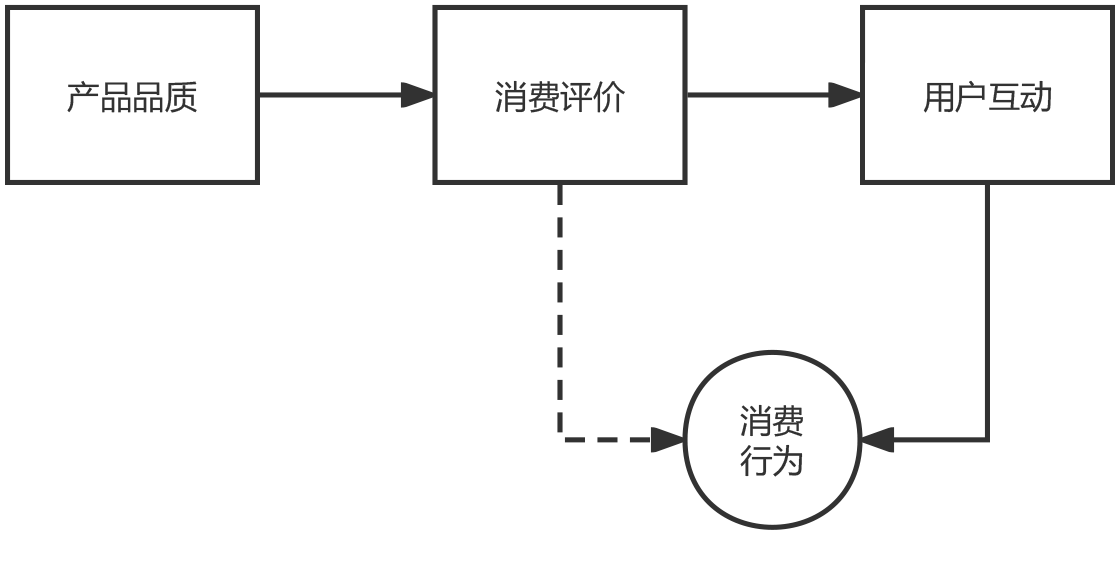
\includegraphics[width=0.6\linewidth]{hw04-imgs/hw04-1.png}
        \caption{研究模型}
        \label{fig:1}
    \end{figure}

    首先,本文验证了产品品质通过影响用户消费评价影响用户消费行为的机制,及用户在直播间的互动行为与用户消费行为的关系。其次,本文将用户的消费评价引入直播间的互动内容中,验证用户会对其他消费者的消费评价产生信任,进而对直播销售的商品产生信任,从而增加直播间的销售量。

    本文使用假设检验的方法进行研究。首先针对产品品质与消费者消费评价之间的关系,我们得到假设$H_1$:

    \begin{hypothesis}
        $H_1$:更高的产品品质会使得消费者消费后给出更高的消费评价
        \label{hyp:1}
    \end{hypothesis}

    其次,当用户在观看商品的直播时,用户由于并未浏览过商品的评论及详情页面,因此对商品的信息主要来自于主播的介绍,因此,消费者在直播间的消费受到产品评价的影响较少。然而,当用户手动浏览商品详情页面时,用户可以自主选择浏览产品评价,因此消费者在商品详情页面的消费受到产品评价的影响较大。由此,我们得到假设$H_{2a}, H_{2b}$:

    \begin{hypothesis}
        $H_{2a}$:当用户自主浏览商品详情页面时,产品的正向评价越多,用户的消费倾向越高。
        \label{hyp:2a}
    \end{hypothesis}
    \begin{hypothesis}
        $H_{2b}$:当用户观看某个商品的直播时,产品的正向评价越多,用户的消费倾向越高。
        \label{hyp:2b}
    \end{hypothesis}

    在假设$H_{2b}$无法显著成立的前提下,我们希望探究将产品评论在直播间展示时,是否会影响用户的消费倾向。由此,我们提出假设$H_{3a}, H_{3b}, H_{3c}$:

    \begin{hypothesis}
        $H_{3a}$:将产品的评价展示在商品的直播间,用户会予以关注。
        \label{hyp:3a}
    \end{hypothesis}
    \begin{hypothesis}
        $H_{3b}$:将产品的评价展示在商品的直播间,会改变用户的消费倾向。
        \label{hyp:3b}
    \end{hypothesis}
    \begin{hypothesis}
        $H_{3c}$:将产品的评价展示在商品的直播间后,产品的正向评价越多,用户的消费倾向越高。
        \label{hyp:3c}
    \end{hypothesis}

    \section{研究方法设计}

    本节说明研究使用的方法,包含问卷调查及行为学实验等。

    \subsection{问卷调查}

    问卷调查部分,我们初步设计了包含(但不限于)如下内容的问卷,问卷以量表的形式呈现,每道题目包含从完全不同意到完全同意的五个选项

    \begin{itemize}
        \item 正常购物部分(即不通过带货直播购物)
        \begin{enumerate}
            \item 我会经常通过淘宝、京东等在线消费平台购物;
            \item 当收到的商品质量不如人意时,我会给差评;
            \item 我在购物时会关注其他人的购买评论,评价越高,我的消费倾向越高;
            \item 我在购物时会\textbf{仅仅}关注其他人的评价,而不在意产品其他方面的水准(如质量,耐用性等)
        \end{enumerate}
        \item 观看带货直播部分
        \begin{enumerate}
            \item 我会经常观看淘宝、京东等平台上的带货直播;
            \item 我会在观看带货直播时从直播间直接下单购物;
            \item 我在从直播间下单商品时,会关注这件商品已有的评价;
        \end{enumerate}
    \end{itemize}

    \subsection{行为学实验}

    行为学实验部分,我们设计了包含如下场景的行为学实验,实验同时使用硬件设备捕捉用户不自主的视觉行为。

    \begin{enumerate}
        \item 被试者分别观看两段直播带货的视频,两段直播带货的视频所指向的商品有不同的消费者评价。在观看后使用量表判断被试的消费倾向。
        \item 被试者分别(或随机)观看三段直播带货的视频,其中一条视频不展示所指向商品的消费者评价;另一条视频将消费者评价嵌入视频内容中;最后一条视频将消费者评价和直播观众的实时互动一并展示。在观看后使用量表判断被试的消费倾向。
        \item 被试者观看三段直播带货的视频,三条视频分别将消费者评价嵌入视频内容中,每条视频中展示相同数量的好评与不同数量的中差评。在观看后使用量表判断被试的消费倾向。
        \item 被试者观看三段直播带货的视频,三条视频分别将消费者和直播观众的实时互动一并展示,每条视频中展示相同数量的好评与不同数量的中差评。在观看后使用量表判断被试的消费倾向。
    \end{enumerate}

    \section{预期结果与潜在创新}

    如前所述,我们预期的实验结果为:

    \begin{enumerate}
        \item 用户会对更高的产品品质给出更好的消费评价,即假设$H_1$成立;
        \item 用户在自主浏览商品详情页面时,会对消费评价给予更多的关注;而用户在观看某个商品的直播时,不会对消费评价给予更多关注,即假设$H_{2a}$成立,假设$H_{2b}$不成立;
        \item 用户会对展示在商品直播间内的消费评价给予关注,并据此调整自身的消费倾向,即假设$H_{3a}, H_{3b}, H_{3c}$成立。
    \end{enumerate}

    本文的潜在创新点在于:通常的直播助农中,商品购买后的评论和购买前的直播互动是独立的,在观看直播时,消费者除了主播外没有其他的额外信息源。本文将购买后的评论引入直播互动中,研究了商品评价对直播观众消费倾向及对产品信任程度的影响,对直播助农中如何更好建立消费者对产品的信任提出了一种新的解决方案。

    \bibliographystyle{gbt7714-numerical}
    \bibliography{HW04}
\end{document}